\documentclass{standalone}
\usepackage{tikz}

\begin{document}
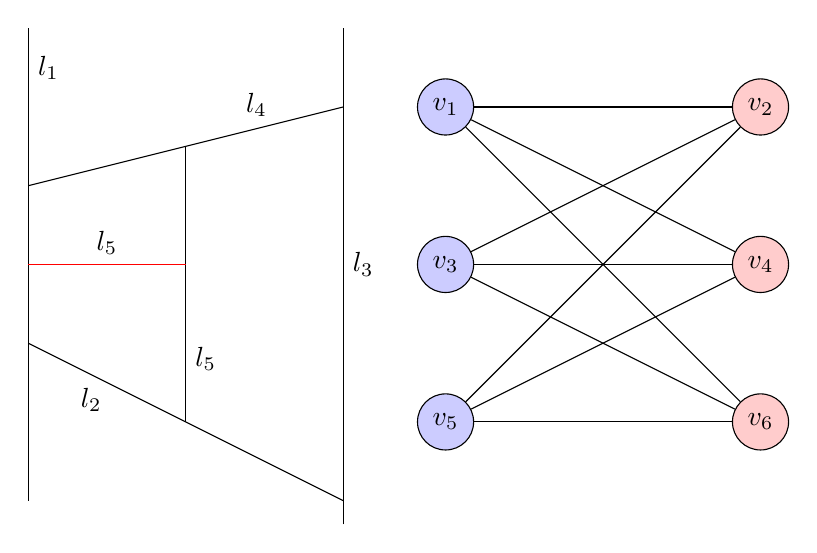
\begin{tikzpicture}
    % Your existing TikZ figure
    % 1
    \draw (0,0) -- (0,6);
    \node[right] at (0,5.5) {$l_{1}$};
    % 2
    \draw (0,2) -- (4,0);
    \node[below] at (0.8,1.55) {$l_{2}$};
    % 3
    \draw (4,-0.3) -- (4, 6);
    \node[right] at (4, 3) {$l_{3}$};
    % 4
    \draw (0, 4) -- (4, 5);
    \node[above] at (2.9, 4.75) {$l_{4}$};
    % 5
    \draw (2, 1) -- (2, 4.5);
    \node[right] at (2, 1.8) {$l_{5}$};
    % 6
    \draw[red] (0, 3) -- (2, 3);
    \node[above] at (1, 3) {$l_{5}$};

    \begin{scope}[xshift=5.3cm]
        % Left side vertices
        \node[circle, draw, fill=blue!20] (L1) at (0, 5) {$v_{1}$};
        \node[circle, draw, fill=blue!20] (L2) at (0, 3) {$v_{3}$};
        \node[circle, draw, fill=blue!20] (L3) at (0, 1) {$v_{5}$};

        % Right side vertices
        \node[circle, draw, fill=red!20] (R1) at (4, 5) {$v_{2}$};
        \node[circle, draw, fill=red!20] (R2) at (4, 3) {$v_{4}$};
        \node[circle, draw, fill=red!20] (R3) at (4, 1) {$v_{6}$};

        % Edges
        \draw (L1) -- (R1);
        \draw (L1) -- (R2);
        \draw (L1) -- (R3);
        \draw (L2) -- (R1);
        \draw (L2) -- (R2);
        \draw (L2) -- (R3);
        \draw (L3) -- (R1);
        \draw (L3) -- (R2);
        \draw (L3) -- (R3);
    \end{scope}

\end{tikzpicture}
\end{document}